\documentclass{beamer}



\mode<presentation>
{
 \usetheme[reversetitle,notitle,noauthor]{Wien} 
%  \usetheme[notitle,noauthor]{Wien} 
}       
  
\usepackage{url}
\usepackage{graphicx}
\graphicspath{{./}{./Figures/}}  

\usepackage{appendixnumberbeamer} 

\usepackage{endnotes} % footnotes at the end of the document

% To avoid a warning from the hyperref package:
\pdfstringdefDisableCommands{%
  \def\translate{}%
}
%%%%%%%%%%%%%%%%%%%%%%%%%%%%%%%%%%%%%%%%%%%%%%%%%%%%%%%%%%%%%%%%%%%%%%%%%%%%% 
%%%%%%%%%%%%%%%%%%%%%%%%%%%%%%%%%%%%%%%%%%%%%%%%%%%%%%%%%%%%%%%%%%%%%%%%%%%%%
\title[SoC Rocket]{SoC Rocket}


%\subtitle{Background Images and Logos\\
%Version 0.5.2}

\author{Johannes Ivancsics\\Florian Muttenthaler\\David Freismuth}


\institute[TU Wien]{TU Wien, Vienna, Austria}
   
\date{\today}


\begin{document}

\begin{frame}
  \titlepage
\end{frame}      


%
% Here is the begin of the SoC Rocket presentation files
%

\begin{frame}{Content}
\begin{itemize}
\item \textbf{Introduction to SoCRocket}
\begin{itemize}
\item Basic Problem
\item Solution
\item Overview and Content of SoCRocket
\end{itemize}
\item \textbf{Transaction Level Modelling}
\begin{itemize}
\item Virtual Platform Model
\item TLM 2.0
\item SoC Rocket Models Library
\end{itemize}
\item David Topics
\end{itemize}

\end{frame}

\begin{frame}{Johannes First slide}
\begin{block}{}
  This is Johannes's first slide
\end{block}
\end{frame}
\begin{frame}{TLM (Transaction Level Modelling)}
\begin{block}{What is TLM?}
	\begin{itemize}
		\item Modelling styles and interoperability rules
  		\item Various levels of details of a design are modelled with one specification language
		\item Raise of abstraction level
	\end{itemize}
\end{block}
\begin{block}{Standard treat two different design issues}
	\begin{itemize}
		\item Communication
		\item Computation
	\end{itemize}	
\end{block}
\end{frame}
\begin{frame}{Virtual Platform Model}
\begin{block}{Purpose}
	\begin{itemize}
		\item TLM for architectural exploration and analysis
		\item Model for developing software applications with a reference model for hardware verification
		\item Available before final RTL exists
\end{itemize}
\end{block}
\begin{block}{Framework}
	\begin{itemize}
		\item Registers and functionality must be accurate
		\item No implementation details like pins or clock
		\item Approximate timing
		\item Fast enough to run software
	\end{itemize}
\end{block}
\end{frame}
\begin{frame}{TLM 2.0}
	\begin{itemize}
		\item OSCI (Open SystemC Initiative) TLM Standard \footnote{\url{https://www.accellera.org/images/downloads/standards/systemc/TLM_2_0_LRM.pdf}}
		\item Purpose Speed and Interoperability
		\item \textbf{Coding Styles:} Loosly Timed and Approximately Timed
	\end{itemize}
\begin{block}{Three Layers}
\begin{figure}
\label{fig:tlm2}
\centering
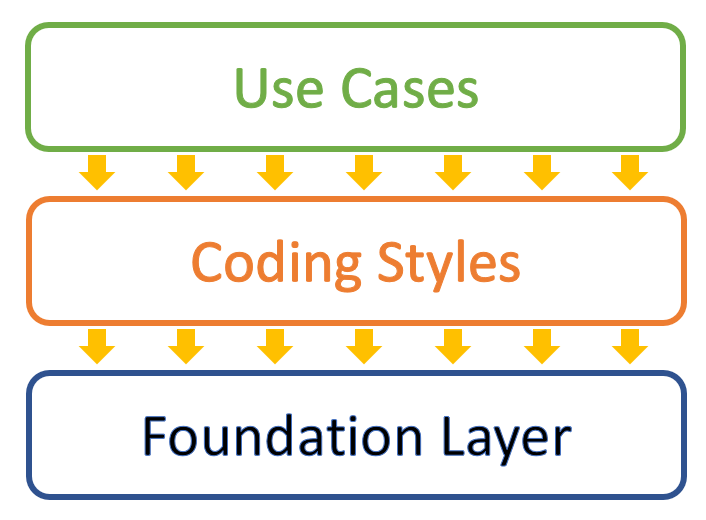
\includegraphics[width=0.5\textwidth]{pictures/Layers.PNG}
\end{figure}
\end{block}
\end{frame}
% \begin{frame}{Coding Styles}
% \begin{block}{Loosely Timed}
% 	\begin{itemize}
% 		\item Simulate as fast as possible
% 		\item Two main methods
% 		\begin{itemize}
% 			\item Temporal Decoupling
% 			\item Use direct memory interface (DMI)
% 		\end{itemize}
% 	\end{itemize}
% \end{block}
% \begin{block}{Approximately Timed}
% 	\begin{itemize}
% 		\item Just accurate enough for performance modelling
% 		\item Processes run in lock step with simulation time
% 	\end{itemize}
% \end{block}
% \end{frame}
\begin{frame}{Interoperability}
\begin{figure}
\label{fig:int}
\centering
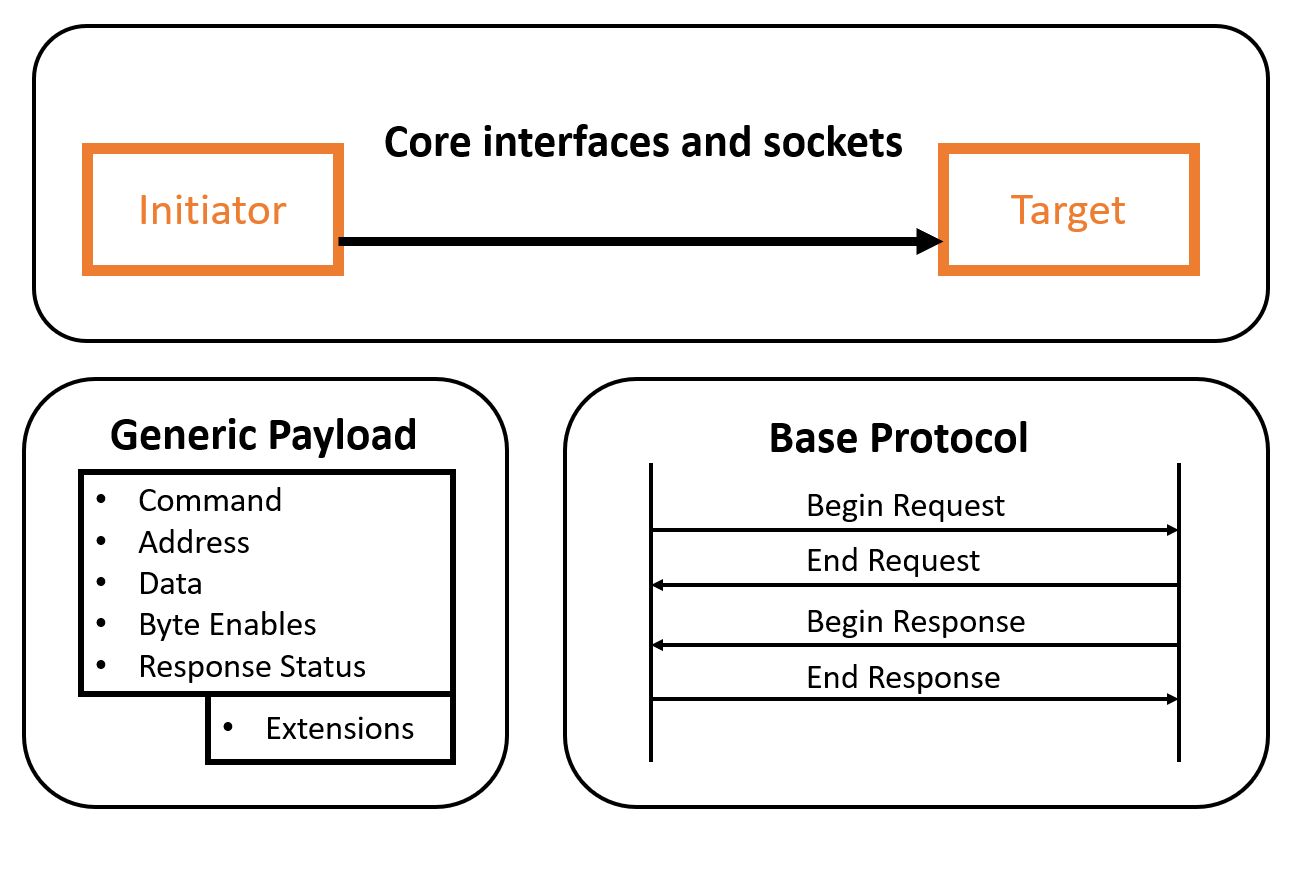
\includegraphics[width=0.9\textwidth]{pictures/Interoperability.PNG}
\end{figure}
\end{frame}
\begin{frame}{SoC Rocket Models Library}
Collection of different IP-Cores written in SystemC under the TLM IEEE Standard\footnote{T. Schuster et al. (2014). SoCRocket - A virtual platform for the European Space Agency's SoC development. 1-7.}
\begin{figure}
\label{fig:Lib}
\centering
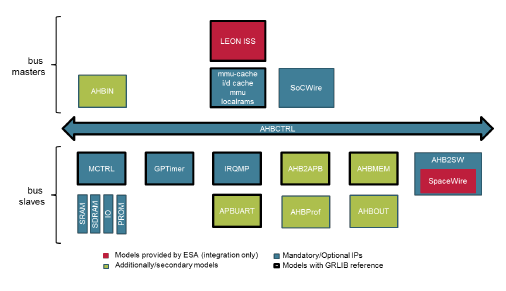
\includegraphics[width=1\textwidth]{pictures/ModelsLibrary.PNG}
\end{figure}
\end{frame}

\begin{frame}{David First slide}
\begin{block}{}
  This is David's first slide
\end{block}
\end{frame}

\begin{frame}{}
  \centering\Huge
  Thank you for your attention
\end{frame}

%
% Here si the begin of the ICT slides
% Useful for syntax help
%
%\begin{frame}{Start of ICT Template}
%\begin{block}{}
%Here is the start of the ICT Template slides. These slides are very useful to learn the syntax.	
%\end{block}
%\end{frame}

%
\begin{frame}{License}
  
\begin{itemize}
\item The TU Wien and ICT logos are covered by copyright rules (see
  \href{www.tuwien.ac.at}{www.tuwien.ac.at}).
\item The rest of the theme is provided under the GNU General Public
  License v. 3 (GPLv3) \href{http://www.gnu.org/licenses/}{http://www.gnu.org/licenses/}. This means that you can redistribute it and/or modify it under the same license. 
\end{itemize}
\end{frame}


%%%%%%%%%%%%%%%%%%%%%%%%%%%%%%%%%%%%%%%%%%%%%%%%%%%%%%%
\begin{frame}{Presentation Template for ICT TU Wien}

  \begin{block}{}
    This theme is designed for presentations of the Instittue of
    Computer Technology (ICT) at the TU Wien, Vienna, Austria.
    \href{www.ict.tuwien.ac.at}{www.ict.tuwien.ac.at}.
  \end{block}

  \vspace{3ex}
  \begin{block}{The theme contains 4 source files}

  \begin{itemize}
  \item  {\tt beamerthemeWien.sty}
  \item  {\tt beamercolorthemeWien.sty}
  \item  {\tt beamerinnerthemeWien.sty}
  \item  {\tt beamerouterthemeWien.sty}
  \end{itemize}
\end{block}
\end{frame} 

%%%%%%%%%%%%%%%%%%%%%%%%%%%%%%%%%%%%%%%%%%%%%%%%%%%%%%%
\begin{frame}{Local and Global Installation}
  
  The theme can be installed for \textbf{local} or \textbf{global} use.
  \begin{block}{Local Installation}
  \begin{itemize}    
    \item Local installation is the simplest way of installing the theme. 
    \item You need to placing the 4 source files in the same folder as
      your presentation. When you download the theme, the 4 theme
      files are located in the {\tt local} folder.
    \item Alternatively you have a local \TeX\  folder under your \texttt{home}
      directory, where \TeX\  finds your packages.
  \end{itemize}
  \end{block}

  \begin{block}{Global Installation}
  \begin{itemize}
     \item If you wish to make the theme globally available, you must
       put the files in your local latex directory tree. The location
       of the root of the local directory tree depends on your
       operating system and the latex distribution.
     \item Detailed steps on how to proceed installation under various
       operating systems can be found in Beamer documentation.
  \end{itemize}
  \end{block}
\end{frame}

%%%%%%%%%%%%%%%%%%%%%%%%%%%%%%%%%%%%%%%%%%%%%%%%%%%%%%%
\begin{frame}{Required Packages}
  \begin{block}{}
    For using the Wien Theme you will need the Beamer class installed
    and the following 4 packages:
    \begin{itemize}
    \item TikZ\footnote{TikZ is a package for creating beautiful
        graphics. Have a look at these
        \href{http://www.texample.net/tikz/examples/}{online examples}
        or the
        \href{http://tug.ctan.org/tex-archive/graphics/pgf/base/doc/generic/pgf/pgfmanual.pdf}{pgf
          user manual}.}
    \item calc
    \item xcolors
    \item tcolorbox
    \end{itemize}
    Due to the fact that the packages are very common they should be
    included in your latex distribution in the first place.
  \end{block}
  \end{frame}

  %%%%%%%%%%%%%%%%%%%%%%%%%%%%%%%%%%%%%%%%%%%%%%%%%%%%%%%
  
\begin{frame}{User Interface}
  \begin{block}{The Presentation Theme}
     The Wien Theme can be loaded in a familiar way. In the preamble
     of your {\tt tex} file you must type\\
     \vspace{5pt}  
    {\tt \textbackslash usetheme[<options>]\{Wien\}}\\ \vspace{5pt} 
    The presentation theme loads the inner, outer and colorWien theme files.
  \end{block}
  \begin{block}{The Inner and Outher Themes}
    If you wish you can load only the color, the inner, or the outer theme directly by\\ \vspace{5pt} 
    {\tt \textbackslash usecolortheme[<options>]\{Wien\}} (it has one option)\\ \vspace{5pt} 
    {\tt \textbackslash useinnertheme[<options>]\{Wien\}} (it has six options)\\ \vspace{5pt} 
    {\tt \textbackslash useoutertheme[<options>]\{Wien\}} (and it has five options)\\
  \end{block}
  
\end{frame}

%%%%%%%%%%%%%%%%%%%%%%%%%%%%%%%%%%%%%%%%%%%%%%%%%%%%%%%
\begin{frame}[fragile]{Package Options - Logos}
   Three options controls the logos on the title frame (Inner Theme option).
  
\begin{itemize}
\item \texttt{logoleft}: Set the logo at the top left position. The default is the file TUW-Logo.png.
\item \texttt{logocenter}: Set the logo at the top centre position. The default is the file no logo.
\item \texttt{logoright}: Set the logo at the top right position. The default is the file ICT-Logo.png.
\end{itemize}

For this presentation I did not change the default logos, so you could either use
\verb| \usetheme[reversetitle,notitle,noauthor]{Wien} |
or
\verb| \usetheme[reversetitle,notitle,noauthor,|
\verb|           logoleft=TUW-Logo.png,|
\verb|           logoright=ICT-Logo.png]{Wien} |


\end{frame}

%%%%%%%%%%%%%%%%%%%%%%%%%%%%%%%%%%%%%%%%%%%%%%%%%%%%%%%
\begin{frame}[fragile]{Package Options - Background}
   Four options control the background images (Inner Theme option).
  
\begin{itemize}
\item \texttt{backgroundfirst}: Set the background image for the first and the last frames. The default is the file TUW-Background.png.
\item \texttt{nobackgroundfirst}: Do not use a background image. The default is to use one.
\item \texttt{backgroundmain}: Set the background image for all body frames. The default is the file ICT-Background.pdf.
\item \texttt{nobackgroundmain}: Do not use a background image. The default is to use one.
\end{itemize}

For this presentation I did not change the default background, so you could either use
\verb| \usetheme[reversetitle,notitle,noauthor]{Wien} |
or
\verb| \usetheme[reversetitle,notitle,noauthor,|
\verb|           backgroundfirst=TUW-Background.png,|
\verb|           backgroundmain=ICT-Background.pdf]{Wien} |

\end{frame}
%%%%%%%%%%%%%%%%%%%%%%%%%%%%%%%%%%%%%%%%%%%%%%%%%%%%%%%
\begin{frame}[fragile]{Package Options - Frame Title}
   One option controls the appearance of the title line on each frame (Outer Theme option).
  
\begin{itemize}
\item \texttt{reversetitle}: Set the frame title to blue and
  foreground to white. The default is a blue font on white background.
\end{itemize}

For this presentation I used

\verb| \usetheme[reversetitle,notitle,noauthor]{Wien} |

\end{frame}
%%%%%%%%%%%%%%%%%%%%%%%%%%%%%%%%%%%%%%%%%%%%%%%%%%%%%%%
\begin{frame}[fragile]{Package Options - Foot Line}
   Four options control the content of the foot line (Outer Theme options).
  
\begin{itemize}
\item \texttt{noauthor}: No author is shown in the central part of the
  foot line.
\item \texttt{notitle}: No title is shown in the central part of the
  foot line.
\item \texttt{noframnumber}: No frame number is shown in the right part
  of the foot line inside the progress circle.
\item \texttt{nocircle}: No progress circle is shown.
\end{itemize}

For this presentation I used

\verb| \usetheme[reversetitle,notitle,noauthor]{Wien} |

\end{frame}

%%%%%%%%%%%%%%%%%%%%%%%%%%%%%%%%%%%%%%%%%%%%%%%%%%%%%%%
\begin{frame}[fragile]{Title Page}

  \begin{block}{}

    The title page can be populated with title, author, institution
    and date. For instance, I used

    \vspace{3ex}

    \hspace{1em}
    \begin{minipage}{0.9\textwidth}
\begin{verbatim}
   \title{ICT Presentations}
   \subtitle{Background Images and Logos }
   \author{Axel Jantsch}
   \institute[TU Wien]{TU Wien, Vienna, Austria}
   \date{\today}

   \begin{document}
   \begin{frame}
     \titlepage
   \end{frame}\end{verbatim}
    \end{minipage}

    \vspace{3ex} to produce the title pages of this presentation.
  \end{block}
\end{frame}


%%%%%%%%%%%%%%%%%%%%%%%%%%%%%%%%%%%%%%%%%
\begin{frame}{}

  \centering\Huge
  !` Enjoy !
\end{frame}

\appendix
%%%%%%%%%%%%%%%%%%%%%%%%%%%%%%%%%%%%%%%%%
\begin{frame}[fragile]{Backup Slides}

  
  \begin{block}{}
    If you have backup slides, the frame numbering is restarted with
    A1, A2, ... for the backup slides, if you use

    
\begin{verbatim}
\usepackage{appendixnumberbeamer}
\end{verbatim}

    in the preamble, and then the command
\begin{verbatim}
\appendix
\end{verbatim}

    after your last slide and before the backup slides. 
  \end{block}

\end{frame}

%%%%%%%%%%%%%%%%%%%%%%%%%%%%%%%%%%%%%%%%%
\begin{frame}{}
  \centering\Huge
  ?` More Questions ?
\end{frame}


\end{document}


%%% Local Variables:
%%% mode: latex
%%% TeX-master: t
%%% End:
